\chapter{Dalla psicologia alla scienza cognitiva}
\section{Lo studio della mente}
Il passaggio dalla psicologia alla scienza cognitiva si fonda principalmente sull’\emph{epistemologia}\index{epistemologia}, ovvero la teoria della conoscenza che studia i principi, i limiti e il metodo della conoscenza scientifica. Negli anni Cinquanta la psicologia cercò di impadronirsi dello studio dei processi mentali attraverso due approcci differenti, il \emph{comportamentismo} e l'\emph{introspezione}.

\subsection{Metodo introspettivo}\index{metodo introspettivo}\index{instrospezione|see{metodo introspettivo}}
L'introspezione è un atto del pensiero che consiste nell'osservazione diretta e nell'analisi della propria interiorità, rappresentata da sentimenti, desideri, prodotti del pensiero stesso, come pure il senso dell'identità di una persona.

La psicologia cognitiva, a partire dagli anni Trenta, ha progressivamente abbandonato l'introspezione come metodo valido per l'indagine, concentrandosi di più sui comportamenti quantificabili piuttosto che sulla coscienza o le sensazioni.

\subsection{Il comportamentismo}
Nella prospettiva di rivoluzionare l'oggetto di studio della psicologia, John Watson\index{Watson, John}\footnote{John Broadus Watson (Greenville, 9 gennaio 1878 – New York, 25 settembre 1958) è stato uno psicologo statunitense, padre del comportamentismo, scuola della psicologia nata dall'osservazione del comportamento degli animali.} attaccò il metodo introspettivo. Egli riteneva l'introspezione un metodo non scientifico per due motivi fondamentali:
\begin{itemize}
  \item l'osservatore si identifica con l'osservato (ad esempio, se l'osservatore osserva la sua coscienza, muta il suo oggetto di osservazione, che coincide con la coscienza di osservare);
  \item la singolarità dell'osservatore conduce all'impossibilità da parte di altri di percepire il medesimo oggetto.
\end{itemize}
In questo modo i dati introspettivi erano solamente percepiti dal singolo, non confutabili o confermabili e non condivisibili come i dati di tutte le altre scienze. Tra il 1913 e il 1939 Watson sviluppa dunque la teoria del comportamentismo, basato sull'assunto che il comportamento esplicito dell'individuo, che è a sua volta riflesso diretto della sua personalità, è l'unica unità di analisi scientificamente studiabile della psicologia, in quanto direttamente osservabile dallo studioso.

La mente viene quindi considerata una sorta di ``black box'', una scatola nera il cui funzionamento interno è inconoscibile e, per certi aspetti, irrilevante: quello che importa veramente per i comportamentisti è giungere ad un'approfondita comprensione empirica e sperimentale delle relazioni tra certi tipi di stimoli (ambientali) e certi tipi di risposte (comportamentali). All'interno di questo ampio approccio, viene posta enfasi su particolari aspetti. Uno degli assunti principali è il meccanismo del \emph{condizionamento}, in base al quale l'associazione ripetuta di uno stimolo, detto \emph{stimolo neutro}, con una risposta che non è ad esso direttamente correlata, farà sì che, dopo un periodo di tempo, a tale stimolo segua la risposta condizionata.

L'esempio classico è fornito dall'esperimento del fisiologo russo Ivan Pavlov\index{Pavlov, Ivan} (figura \ref{fig:pavlov}), il primo autore che ha identificato il meccanismo, che faceva precedere alla somministrazione del cibo a dei cani un suono; con il tempo il cane apprende che, dopo il suono, gli verrà fornito il cibo; a seguito del condizionamento, il suono di per sé generava la salivazione del cane. Lo stimolo neutro, non in grado di determinare la risposta condizionata (la salivazione), dopo tale ripetuta associazione, determina la risposta condizionata. Alcuni comportamentisti sostengono semplicemente che l'osservazione del comportamento è il modo migliore, o il più conveniente, per investigare i processi psicologici e mentali.

\begin{figure}[hbt]
  \centering
  \includegraphics[width=0.9\textwidth]{img/cani_Pavlov.jpg}
  \caption{I cani di Pavlov.}
  \label{fig:pavlov}
\end{figure}

\section{La nascita del funzionalismo}
I due approcci allo studio della mente erano entrambi inadatti; l’approccio comportamentista osserva solo lo stimolo e la reazione, ovvero l’input e l’ouput, e non i processi mentali intermedi che li correlano. Inoltre, la relazione fra stati mentali e comportamenti non può essere considerata lineare (ad esempio, persone diverse nello stesso stato mentale possono avere comportamenti diversi).

L’introspezione d’altra parte è metodologicamente debole. Inferire gli stati mentali osservando sé stessi è un approccio sbagliato, in quanto noi riusciamo a cogliere ciò che ci aspettiamo: l’aspettativa domina l’osservazione e non siamo in grado di controllare la correttezza delle intuizioni perché è impossibile l’\emph{itersoggettività}\index{intersoggettività} (ovvero poter ripetere l’esperimento cambiando il soggetto).

È pertanto necessario adottare una metodologia in grado di rispondere a criteri di scientificità aggirando l’ostacolo della non osservabilità. Questo può avvenire grazie all’informatica e all’intelligenza artificiale. La funzione mentale in esame resta inosservabile, ma riuscire a riprodurla completamente può permettere di introdurre criteri operativi di scientificità in grado di sostituirsi a quelli basati sull’osservabilità.

L’esperimento richiede dunque l’intersoggettività (chiunque deve poter ripetere l’esperimento, che non deve essere legato a caratteristiche particolari, personali e non comunicabili) e la \emph{riproducibilità} (l’esperimento deve poter essere ripetuto a piacimento, variando tutte le condizioni che non siano state esplicitamente poste come ineliminabili).

Nel caso specifico dello studio della mente però, resta aperto il problema della riproducibilità: come si può decidere quando un determinato fenomeno è stato riprodotto? Una importante chiarificazione arriva dalla corrente filosofica del funzionalismo\index{funzionalismo}. Secondo Hilary Putnam\index{Putnam, Hilary}, principale rappresentante di questa corrente, la struttura fisica che produce un determinato fenomeno è irrilevante se al livello di analisi scelto non ci sono differenze significative fra l’originale e il riprodotto. Così, che un processo di ragionamento sia realizzato da un sistema biologico come il cervello oppure da un sistema elettronico come un calcolatore, non implica che ci sia una differenza fra i due processi.

\section{Funzionalismo e modularità}
Il funzionalismo\index{funzionalismo} è una teoria della mente, sviluppata da Hilary Putnam\index{Putnam, Hilary} nel 1950, in contrapposizione al riduzionismo materialista (e.g. la teoria dell'identità) e al comportamentismo per superare la diatriba mente-corpo nella filosofia della mente contemporanea.

L'idea di base è che gli stati mentali (desideri, convinzioni, ecc) siano costituiti solamente dal loro ruolo, cioè dalla loro funzione, la loro relazione causale, rispetto ad altri stati mentali, percezioni e comportamento. Giacché gli stati mentali possono essere definiti in base al loro ruolo funzionale, essi sono molteplicemente realizzabili; in altre parole, possono manifestarsi in vari sistemi, anche artificiali (e.g. calcolatori), se il sistema computa le funzioni adatte. L'analogia mente/computer, che vede il cervello paragonato all'hardware e la mente al software, costituisce l'emblema di gran parte delle teorie funzionaliste della mente.

Le prime forme di funzionalismo furono proposte da Hilary Putnam (che poi abbandonerà tale approccio) e da Jerry Fodor\index{Fodor, Jerry} negli anni Sessanta. L'argomento chiave che utilizza Putnam per sostenere la superiorità del paradigma funzionalista è la cosiddetta \emph{teoria delle molteplici realizzazioni}\index{molteplici realizzazioni, teoria delle}: è impossibile identificare mente e cervello in quanto diversi stati cerebrali possono comportare il medesimo stato mentale.

Il funzionalismo di Fodor si pone ad un livello di analisi più profondo di quello di Putnam: egli considera sbagliato fermarsi a considerare l'aspetto funzionale della mente in termini di macroelaborazione di input e output. Secondo Fodor sono gli stati mentali interni ad essere organizzati funzionalmente secondo proprietà semantiche e relazioni sintattiche tra loro, con gli stati neuronali che implementano in modi diversi tali stati mentali.

La \emph{teoria della mente modulare}\index{mente modulare} di Fodor (1983) ha avuto un notevole impatto sui ricercatori interessati allo studio dello sviluppo cognitivo, perché ha suggerito l'esistenza di un forte legame tra la tesi innatista e il carattere dominio-specifico della cognizione, descrivendo l'architettura della mente come vincolata da un'architettura innata, rigida e immutabile, altamente dominio-specifica.

Secondo Fodor, infatti, l'architettura della mente è costituita, fin dalla nascita, da un insieme di elaboratori altamente efficienti e specializzati, i moduli\index{moduli cognitivi}, che codificano e manipolano specifici tipi di informazioni, e la cui presenza è specificata nelle istruzioni genetiche. Nel corso della filogenesi (storia dell’uomo), gli esseri umani avrebbero sviluppato sistemi di elaborazione dell'informazione che hanno permesso loro di dare un senso al mondo in cui si sono evoluti.

Fodor attribuisce un grande ruolo all'ambiente nello sviluppo dei moduli cognitivi a livello filogenetico, ma non a livello ontogenetico (storia di una singola persona – la mente avrebbe sviluppato la sua architettura modulare come forma di adattamento ad esso, nel corso dell'evoluzione).

La mente umana è quindi formata da 3 componenti:

\begin{description}
	\item [trasduttori] trasformano le informazioni contenute nello stimolo in un formato manipolabile dal sistema cognitivo, ricevute dai sistemi di input, e forniscono ai sistemi centrali la rappresentazione del mondo esterno;
	\item [moduli (sistemi di input)] decodificatori automatici delle informazioni presenti nell'ambiente; ricevono l'input dai trasduttori; attraverso i moduli, la mente trasforma gli stimoli ambientali in rappresentazioni, in modo automatico, guidata dal basso a partire dalle condizioni di stimolazione;
	\item [sistemi centrali] funzioni superiori, come pianificazione del comportamento, problem solving, ecc; operazioni lente, sotto controllo volontario e cosciente, influenzate dagli scopi cognitivi globali che il soggetto si pone.
\end{description}
 
Secondo Fodor, i moduli possono essere collocati tra le visioni comportamentiste e cognitiviste dei processi di basso livello. I comportamentisti cercarono di rimpiazzare la mente con i riflessi che Fodor descrive come incapsulati\index{impenetrabilità cognitiva} (impenetrabili, ovvero non affetti da altri domini cognitivi) e non inferenziali. Al contrario, i cognitivisti vedono i processi di basso livello un continuo con i processi di alto livello, inferenziali e penetrabili cognitivamente. Quest’ultima affermazione è stata smentita in alcuni casi, come negli esempi delle illusioni ottiche, nelle quali l’effetto resta anche con la consapevolezza dell’illusione. Questo fatto indica che altri domini, incluso ciò che sappiamo, non possono influenzare questi processi. Fodor arriva quindi alla conclusione che questi processi sono inferenziali come i processi di alto livello, ma incapsulati allo stesso modo dei riflessi.

Nonostante Fodor sostenesse la modularità dei processi cognitivi di basso livello, affermò anche che i processi di alto livello non sono modulari, in quanto essi hanno proprietà differenti. I sistemi modulari devono infatti soddisfare determinate proprietà:
\begin{itemize}
  \item specificità del dominio, i moduli operano solo su determinati input e sono altamente specializzati;
  \item isolamento informazionale, i moduli non necessitano di comunicare con latri sistemi psicologici per funzionare;
  \item non interrompibili, i moduli processano in modo mandatorio;
  \item molto veloci, probabilmente dovuto al fatto di essere impenetrabili e mandatori;
  \item semplicità dell’output;
  \item accessibilità limitata;
  \item ontogenesi caratteristica;
  \item architettura neurale fissa.
\end{itemize}

Nel 1999 Pylyshyn\index{Pylyshyn, Zenon} sostenne che mentre queste proprietà tendono a manifestarsi con i moduli, una soltanto, l’impenetrabilità, può essere considerata come distintiva di un modulo, poiché isola i processi dentro al modulo dalle influenze esterne e dagli accessi di altri sistemi. Un classico esempio è costituito dall’illusione di Müller-Lyer\index{illusione di Müller-Lyer}, proposta da Franz Carl Müller-Lyer (1857–1916), un sociologo tedesco, nel 1889, per il fatto che la consapevolezza dell’illusione non corregge il processo visuale.

\begin{figure}[hbt]
  \centering
  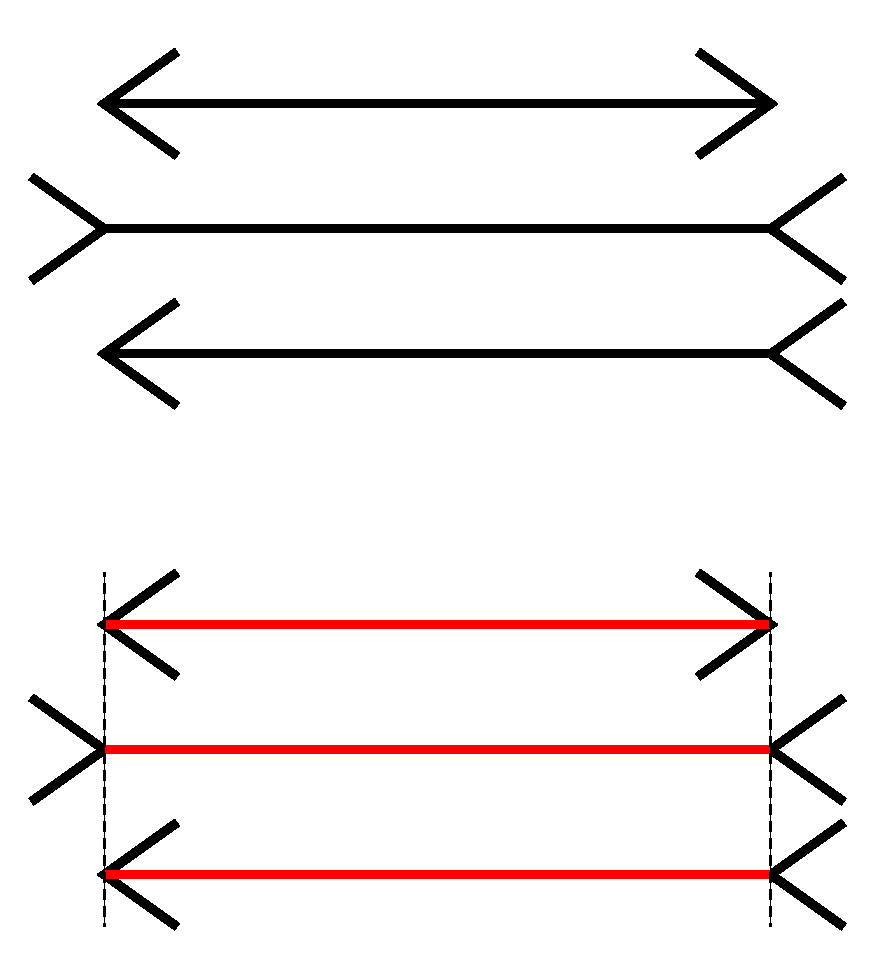
\includegraphics[width=0.5\textwidth]{img/Muller-Lyer_illusion}
  \caption{Due insiemi di linee che mostrano l'illusione ottica di Müller-Lyer.}
  \label{fig:illusioneMuller}
\end{figure}

Un esempio di illusione di Müller-Lyer è proposto nella figura \ref{fig:illusioneMuller}: la lunghezza delle linee è sempre la stessa, ma i riferimenti angolari fanno percepire proporzioni differenti al cervello umano. Il secondo insieme di linee mostra, tramite le linee tratteggiate, l'equivalenza dei segmenti. Nonostante questa consapevolezza, l'illusione di vedere righe di dimensioni differenti permane.

\subsection{Rivalutazione del comportamentismo}
L'ultima cosa da chiedersi nello studio di una funzione cognitiva, è a che livello di dettaglio arrestarsi nello scomporre la funzione in moduli più semplici. La risposta arriva dallo psicologo Robert Cummins\index{Cummins, Robert}, che propone di fermarsi quando i processi sono così semplici che possono essere direttamente implementati, ovvero possono essere considerati ``hardwired'' nel cervello. Solo a questo livello di dettaglio la teoria del comportamentismo può essere considerata valida, in quanto il modulo può essere visto come la ``black box'' che reagisce agli stimoli producendo una risposta. 

\section{L'unità TOTE}\index{unità TOTE}
Il lavoro più significativo che porta la psicologia ad incidere e influenzare la scienza cognitiva è quello di George Miller\index{Miller, George}\footnote{George Armitage Miller (Charleston, 3 febbraio 1920 – Plainsboro, 22 luglio 2012) è stato uno psicologo statunitense. È stato uno dei fondatori e massimi esponenti storici della psicologia cognitiva. È noto anche per aver gettato le basi della psicolinguistica, con il testo Linguaggio e comunicazione (1951).} (psicolinguista), Galanter (psicologo matematico) e Pribram (neuropsicologo). Nel 1960 produssero il testo \emph{Plans and structure of behaviour}, nel quale si evidenzia che il comportamento è un processo organizzato su più livelli. Al fine di raggiungere un obiettivo l’uomo elabora un piano, che viene definito come un processo comportamentale gerarchico che controlla l’ordine in cui deve essere eseguita una sequenza di operazioni. In ogni istante l’organismo che elabora ed esegue il piano possiede una conoscenza organizzata, ovvero un’immagine di sé stesso e del mondo. Di fatto tutto questo è l’equivalente di un programma per il calcolatore.

Questi elementi permettono di definire quella che viene considerata l’unità elementare del comportamento: il circuito a feedback TOTE (Test-Operate-Test-Exit), mostrato nella figura \ref{fig:tote}.

\begin{figure}[hbt]
  \centering
  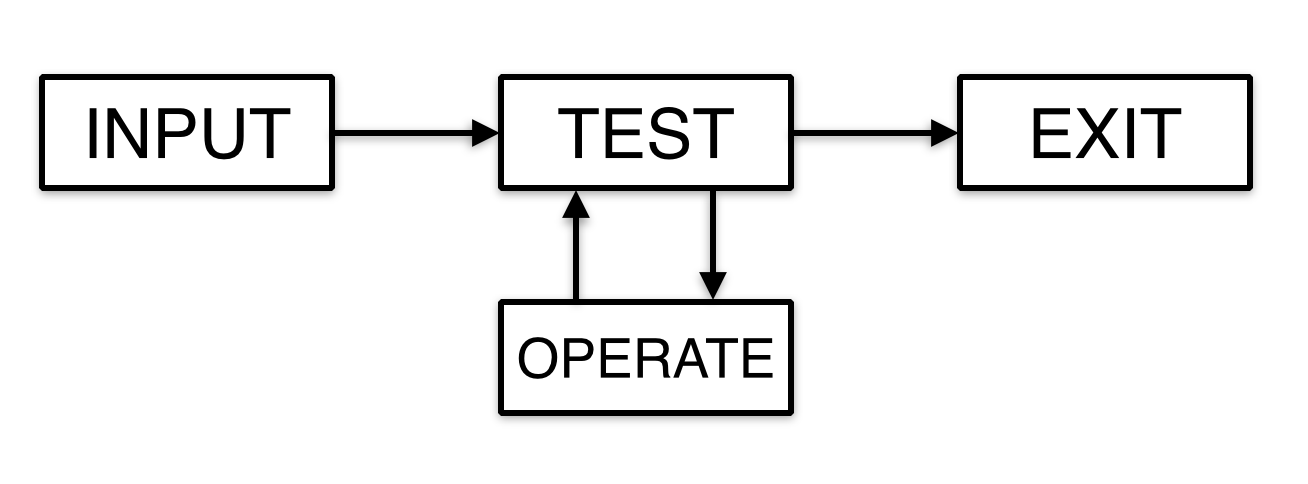
\includegraphics[width=\textwidth]{img/TOTE.png}
  \caption{Schema dell'unità TOTE}
  \label{fig:tote}
\end{figure}

Il punto di partenza è lo stato iniziale del mondo; il primo passo consiste nel chiedersi se questo coincide con lo stato desiderato. Se non lo è, si effettuano delle operazioni per diminuire la differenza tra lo stato attuale e quello desiderato, si effettua nuovamente il test e si ripete questa iterazione finché non si ottiene lo stato finale e quindi la risposta positiva, che consente l’uscita e l’arresto dell’azione. L’esempio più noto di unità TOTE è il compito di piantare un chiodo: si parte con il chiodo fuori dal muro e si batte la testa con il martello finché non si raggiunge il livello di penetrazione desiderato. A quel punto l’azione si interrompe e l’obiettivo è raggiunto.

Un piano d’esecuzione può comprendere più unità TOTE, che si possono correlare secondo un’organizzazione gerarchica rispettante la struttura del circuito a feedback negativo atto a diminuire le differenze fra lo stato attuale e quello desiderato.

Questa analisi del comportamento diede un forte contributo allo sviluppo della scienza cognitiva: il TOTE è infatti immediatamente traducibile in un programma di calcolo e questo aprì la strada alla simulazione su computer del comportamento umano.

\section{Concetti e categorie}
Uno degli psicologi più vicini alla scienza cognitiva è Jerome Bruner, che con i suoi studi sulla percezione sottolinea come essa sia influenzata dalla posizione sociale e dalla personale esperienza di chi le percepisce.

Nel 1956, nell’opera \emph{A study of thinking} costituisce la prima teorizzazione unitaria sui processi del pensiero, confermate poi nel 1966 in \emph{Studies in cognitive growth}. Vengono studiati i processi di comprensione dei concetti, ed in particolare come si formino e si applichino le strategie utili ad apprendere nuovi concetti. Burner confutò il precedente approccio probabilistico che legava l’apprendimento ad un processo meccanico di calcolo.

La comprensione di un concetto implica una catena di decisioni successive, di cui le prime influenzano i gradi di libertà possibili per le decisioni successive. I procedimenti che permettono di comprendere un concetto, chiamati strategie, hanno diversi scopi: assicurarsi che il concetto sia raggiunto dopo un numero minimo di incontri con casi rilevanti, assicurarsi che il concetto abbia un alto grado di certezza, ridurre al minimo lo sforzo cognitivo relativo all’inferenza e alla memoria, ridurre al minimo il numero di categorizzazioni sbagliate.